\documentclass[a4paper]{article}
\usepackage{caption}
\usepackage{subcaption}
\usepackage{tikz}
\usetikzlibrary{bayesnet}
\usepackage{booktabs}




\setlength{\tabcolsep}{12pt}
\begin{document}
	
	
	
	



	
	\begin{figure}[ht]
		\begin{center}
			\begin{tabular}{@{}c|c@{}}
				\toprule
				
				Plate Notation &  Factor\\  \midrule
				&                             \\
				
					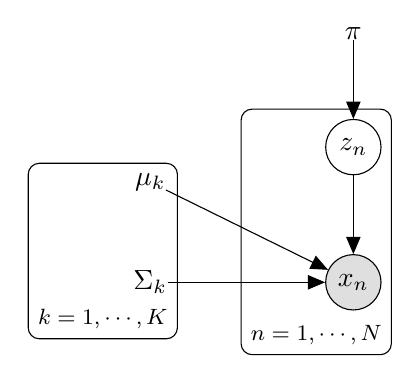
\begin{tikzpicture}
					\node[obs]                               (xn) {$x_n$};
					\node[latent, above=of xn]                               (zn) {$z_n$};
					\node[const, above=of zn]                               (pi) {$\pi$};
					
					\plate{}{(xn)(zn)}{$n = 1, \cdots, N$};
					
					\node[const, left=2cm of xn]                               (sigmak) {$\Sigma_k$};
					\node[const, above=of sigmak]                               (muk) {$\mu_k$};
					
					\plate{}{(sigmak)(muk)}{$k = 1, \cdots, K$};
					
					\edge {muk,sigmak,zn} {xn} ; %
					\edge {pi} {zn};
					
					
				\end{tikzpicture}
				
				
	&
							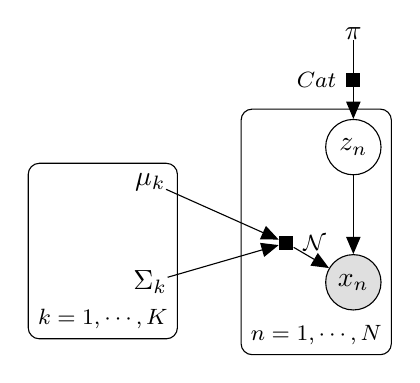
\begin{tikzpicture}
				\node[obs]                               (xn) {$x_n$};
				\node[latent, above=of xn]                               (zn) {$z_n$};
				\node[const, above=of zn]                               (pi) {$\pi$};
				
				\plate{}{(xn)(zn)}{$n = 1, \cdots, N$};
				
				\node[const, left=2cm of xn]                               (sigmak) {$\Sigma_k$};
				\node[const, above=of sigmak]                               (muk) {$\mu_k$};
				
				\plate{}{(sigmak)(muk)}{$k = 1, \cdots, K$};
				
				
				\edge {pi} {zn};
				
				\factor[above=of zn] {z-f} {left:${Cat}$} {} {} ; %
				\factor[left=of xn,yshift=0.5cm] {x-f} {right:$\mathcal{N}$} {} {} ; %
				
				\edge {muk,sigmak} {x-f} ; %
				\edge {x-f,zn}{xn};
				
			\end{tikzpicture}
			
				
			\end{tabular}
			
		\end{center}
		\caption{Graphical models for Gaussian Mixture Model}
	\end{figure}

	
\end{document}